\chapter{Applications}
\label{sec:apps}
As described in Section \ref{ch:intro}, IVCs can facilitate several engineering tasks in different phases of a system development process. This chapter explains some of the IVC applications we have explored.
\iffalse
Safety-critical systems, like an airborne software, must undergo a rigorous software development process usually governed by particular standards, such as DO-178C for Software Considerations in Airborne Systems and Equipment Certification \cite{DO178C} and DO-333 for Formal Methods Supplement to DO-178C and DO-278A \cite{DO333}.
DO-178C proposes a rigorous software development process that starts with an abstract requirements artifact that is iteratively refined into a software designs, source code, and finally, object code, and a set of {\em objectives} that should be met by critical avionics software.  Two of the key tenets of this process are traceability and adequacy; that is, each refinement of an artifact must be traceable to the artifact if was derived from. Further, each refinement must be shown not to introduce functionality not present in the artifact from which it was derived (adequacy). For example, DO-178C objectives A-3.6 (traceability of high-level requirements to system requirements) and A-4.6 (traceability of software design to high-level requirements) specifically require applicants to demonstrate bi-directional traceability.

DO178C currently uses a variety of metrics to determine adequacy of requirements, but much of the effort involves code-level testing.  Test suites are derived from requirements and used to test the software and measured using different structural coverage test metrics.  If code-level test suites do not achieve full coverage, then an analysis is performed to determine whether there are missing requirements and test cases.  The kind of structural coverage required (e.g., statement, branch, MCDC) for adequate testing is driven by the criticality of the software in question.

The utility of the IVCs are being evaluated by Rockwell Collins on a pilot project for both traceability and adequacy checking \cite{lucas17}. Previously, bi-directional traceability between artifacts involved tedious manual peer review to determine that requirements were adequate and that additional functionality was not introduced in the implementation model. IVCs offer automation to satisfy the DO178C objectives related to traceability and adequacy, which is a very important use in providing certifications. This section describes how IVCs can be employed for traceability and adequacy checking.
\fi

\section{Automatic Proof-Based Traceability}
\label{sec:traceability}

\section{Preliminaries}
\label{sec:background}
\newcommand{\satisfies}{\vdash_{\!\!s}}
\newcommand{\nsatisfies}{\nvdash_{\!\!s}}
\newcommand{\bool}[0]{\mathit{bool}}
\newcommand{\reach}[0]{\mathit{R}}
\newcommand{\ite}[3]{\mathit{if}\ {#1}\ \mathit{then}\ {#2}\ \mathit{else}\ {#3}}
\newcommand{\nondetcov}{\text{\sc Nondet-Cov}}
\newcommand{\mutcov}{\text{\sc Mutant-Cov}}

\subsection{Models, Requirements, and Provability}

We define \emph{provability} of a requirement with respect to a model independent of a particular proof system.  We define the implementation model as a set of formulas $\Gamma$  and the set of requirements $\Delta$.
Then given $\Gamma' \subseteq \Gamma$ and $\delta \in \Delta$, we use the notation $\Gamma' \vdash \delta$ to mean that $\delta$ is \emph{provable} given the set $\Gamma'$.  We assume that the provability relation $\vdash$ is monotonic on the subset relation over $\Gamma$, that is, if $\Gamma'' \subseteq \Gamma' \subseteq \Gamma$ and $\Gamma'' \vdash \delta$, then $\Gamma' \vdash \delta$.  The monotonicity of the satisfaction relation means that, unless {\em all} elements of the implementation $\Gamma$ are required for a proof, there are multiple implementation sets $\Gamma'' \subset \Gamma' \subset \ldots \subset \Gamma$ that can satisfy a given requirement $\delta$.  In an abuse of notation, we write $\Gamma' \vdash \Delta$ to mean the conjunction of all requirements in $\Delta$: $\Gamma' \vdash \bigwedge \Delta$.

\subsubsection{Example: Transition Systems}
\label{sec:ts}
We can straightforwardly instantiate our abstract model over a transition system for proving safety properties.  Given a state space $S$, a transition system $(I,T)$ consists of an initial state predicate $I : S \to \bool$ and a transition step predicate $T : S \times S \to \bool$. We define the notion of reachability for $(I, T)$ as the smallest predicate $\reach : S \to \bool$ which satisfies the following formulas:
\begin{gather*}
  \forall s.~ I(s) \Rightarrow \reach(s) \\
  \forall s, s'.~ \reach(s) \land T(s, s') \Rightarrow \reach(s')
\end{gather*}
A safety property $P : S \to \bool$ is a state predicate. A safety property $P$ holds on a transition system $(I, T)$ if it holds on all reachable states, i.e., $\forall s.~ \reach(s) \Rightarrow P(s)$, written as $\reach \Rightarrow P$ for short. When this is the case, we write $(I, T)\vdash_{T} P$, for provability within the transition system.  We assume the transition relation of the system has the structure of a top-level conjunction. This assumption gives us a structure that we can easily manipulate. Given $T(s, s') = T_1(s, s') \land \cdots \land T_n(s, s')$ we will write $T = T_1 \land \cdots \land T_n$ for short. By further abuse of notation we will identify $T$ with the set of its top-level conjuncts. Thus we will write $x \in T$ to mean that $x$ is a top-level conjunct of $T$; or, equivalently, $\Gamma = \{T_1, T_2, \ldots, T_n\}$ and $\Delta = \{P\}$ in our abstract model.

Such a transition system can easily encode our example model in Section~\ref{sec:example}.  We assume each equation defines a conjunct within the transition system which we will denote by the variable assigned, so $\Gamma = \{$ {\small \texttt{a1\_below, a2\_below, a1\_above, a2\_above, below, above\_hyst}} $\}$.
%\footnote{In the example in Section \ref{sec:example}, $\Gamma = \{{\tt P}, {\tt x}, {\tt c1}, {\tt c2}, {\tt c3}, {\tt r1}, {\tt r2}\}$ and $\Delta = \{{\tt P}\}$.}

%Such transition systems can represent either finite or infinite state systems, depending on the state space $S$.

%We will write $S \subseteq T$ to mean that all top-level conjuncts of $S$ are top-level conjuncts of $T$. We will write $T \setminus \{x\}$ to mean $T$ with the top-level conjunct $x$ removed.


%\paragraph{Applying Provability to Transition Relations and Safety Properties}

%\mike{To do: add a few paragraphs on instantiating the formal model for transition systems and model checking (a la IVCs), then further elaborate it for Netlists (a la Chockler and Kroening).}

%\mike{We could cover tableau methods here, but these are overly restrictive}

\subsection{Requirements Coverage and Mutations}
The goal of a coverage metric is usually to assign a numeric score that describes how well requirements cover the design.  The majority of the work in requirements coverage metrics has focused on {\em mutations}, which are ``atomic'' changes to the design, where the set of possible mutations depends on the notation that is used.  A mutant is ``killed'' if one of the requirements that is satisfied by the original design is violated by the mutated design~\cite{chockler_coverage_2003,chockler2001practical,chockler2010coverage,Kupferman:2006:SCF,kupferman_theory_2008}.  There are Many different kinds of mutations that have been proposed, primarily focused on checking sequential bit-level hardware designs.  For these designs, {\em State-based} mutations flip the value of one of the bits in the state.  There are several variations depending on whether the flip is performed on a single state within a Kripke structure~\cite{hoskote1999coverage}, or in the description of the signal in the transition relation of the circuit~\cite{chockler2001practical}.  {\em Logic-based} mutations fix the value of a bit to constant zero or one, and can be used to determine whether requirements can find stuck-at faults.  {\em Syntactic} mutations~\cite{chockler_coverage_2003} remove states in a control flow graph representation of hardware.  Similarly, for software, it is possible to apply any of the ``standard'' source code mutation operators used for software testing~\cite{Andrews06:mutation} towards requirements coverage analysis.  Some examples of software mutations are: 
\begin{enumerate}
    \item Replace an integer constant C by one of $\{0, 1, -1, C + 1, C - 1\}$.
    \item Replace an arithmetic, relational, logical, bitwise logical, increment/decrement, or arithmetic-assignment operator by another operator from the same class.
    \item Negate the decision in an if or while statement
    \item Delete a statement
\end{enumerate}


For our abstract model, we assume each element $\gamma \in \Gamma$ has a set of possible mutations associated with it.  Depending on the modeling formalism used, this may be the value of a gate or signal or an expression within a statement in a program.  We will further assume the existence of a mutation function $f_{m}$ that, given a model element, will return a finite set of mutations for that element.  We can then define the set of mutant models $M$ as follows:
\[
    M = \{ \gamma \in \Gamma, m \in f_{m}(\gamma)\ |\ \Gamma - \{\gamma\} \cup \{m\} \}
\]

\noindent and then define the mutation score for a set of requirements $\Gamma$ in the standard way:

\begin{definition} {\emph{Generalized mutation coverage.} } \\
\[
   \mutcov = \frac{ | \{m \in M(\Gamma)~|~ m \nvdash \Delta\} |}{|M(\Gamma)|}
\]
\end{definition}

%\mike{Do we want these parameterized?  We could just assume Gamma and Delta}

In our example in Figure~\ref{fig:asw}, applying the software mutations from~\cite{Andrews06:mutation} would involve manipulating the constants used in the definitions of \texttt{a1\_below, a2\_below, a1\_above, a2\_above}, swapping 'or' and 'and' in the definition of \texttt{below, above\_hyst}, or negating the conditions in the if/then/else statements.  Even for this small model, note that there are a large number of possible mutations: 57 given the set defined above, and that this number increases rapidly with the size of the program and the chosen set of mutations.


%\mike{Illustrate on running example here.}

Of particular interest is the mutation that replaces a computed variable ({\em signal} in hardware) with a ``fresh'' input; this mutation is called a {\em nondeterminism mutation} with a coverage metric called (\nondetcov)~\cite{chockler2010coverage} and is discussed in~\cite{Kupferman:2006:SCF,kupferman_theory_2008,chockler2010coverage}.  If we use an equational transition system to assign the variables, then performing \nondetcov\ coverage an isomorphic operation to removing the defining equation from the set $\Gamma$ and checking whether provability is preserved.  In this case, we can dispense with the set $M$ and compute a mutation score much more simply:

\begin{definition} {\emph{Nondeterministic coverage.} }
\[
   \nondetcov = \frac{ | \{\gamma \in \Gamma~|~ \Gamma - \{\gamma\} \nvdash \Delta\} |}{|\Gamma|}
\]
\end{definition}

\noindent In one sense, the nondeterminism mutation is the {\em strongest} mutation because it introduces the most additional behaviors into the model, that is, any execution sequence constructed by modifying the assigning equation is also an execution sequence for a nondeterministic mutation.  Equivalently, given a set of universal properties, it is the easiest mutation to ``kill''.  For our example in Figure~\ref{fig:asw}, this mutation would lead to 10 mutations, one for each equation in the model.

%\mike{Illustrate on running example here}

\iffalse
\subsection{Requirements Coverage and Structural Testing}
\mike{not sure we need this...if so, we need to accurately characterize test obligations as a function from elements in $\Gamma$}
In {\em black-box} testing, one is interested in creating a suite of tests from requirements that adequately exercise the behavior
of a software system without regard to the internal structure of the implementation.  This is the preferred style of testing in
safety-critical domains and is advocated by standards such as DO-178B~\cite{RTCA:DO-178B}.  The adequacy of such test suites are usually inferred by examining different coverage metrics on an executable artifact, either source code~\cite{Bezier90:TestingBook,MCDCPaper} or software models~\cite{Ammann99:SpecBasedCoverageMetric,Sanjai03:dissertation}.  If the tests are not sufficient to cover the structure of the code, then either additional tests are derived from existing requirements, or (often) additional requirements are created to describe the additional functionality that is not covered by any tests.

Common metrics used for test coverage measurement are {\em statement}, {\em decision}, and {\em modified condition/decision coverage (MCDC)}.  In this section, we use the rigorous MCDC metric to measure coverage.  \mike{Define MCDC}.

It is straightforward to define coverage in a way that is parametric to the particular test metric that is used.  Given a set $\Theta$ of all possible tests and $\Phi$ the set of all {\em test obligations} induced by the test metric over the model, we define three functions.  The first, $R_m : \Delta \rightarrow 2^\Theta$, defines the set of tests furnished for each requirement.  The second, $E_m : \Gamma \rightarrow 2^\Phi$ defines the test obligations associated with each model element.  The third, $T_m : \Theta \rightarrow 2^\Phi$, defines the obligations that are covered by the test.  Then coverage can be defined as: $$\frac{|\bigcup_{t \in T} T_m (t)|}{|\Phi|}$$.


%Formally, irrespective of the metric used, given $T$ the set of all tests, and the user furnishes test cases associated with each requirement: . Coverage for a given test is measured using a function that maps tests to model elements  as follows \cite{chelenski1994oapplicability, schuler_assessing_2011, murugesan2015we}: $$\frac{|\bigcup_{t \in T} T_m (t, \Gamma)|}{|\Gamma|}$$

%
%\mike{revise}
%

A common problem with this metric is masking:
the effect of a change in a variable cannot be observed in the output. To illustrate, consider the example in Fig. \ref{fig:ex}; suppose we are provided with
test suite \{\{{\tt in1} = \emph{true}, {\tt in2} = \emph{false}\},
\{{\tt in1} = \emph{false}, {\tt in2} = \emph{false}\}\}. The change in the value of
{\tt in1} is masked by {\tt c1}. This problem causes the coverage method reports something covered
while it actually does not affect the output at all.



%\noindent In the following sections, we will examine other possible scoring mechanisms based on minimal provability, and contrast them against testing and vacuity-based metrics.

%\begin{figure}[htb]
%\begin{center}
%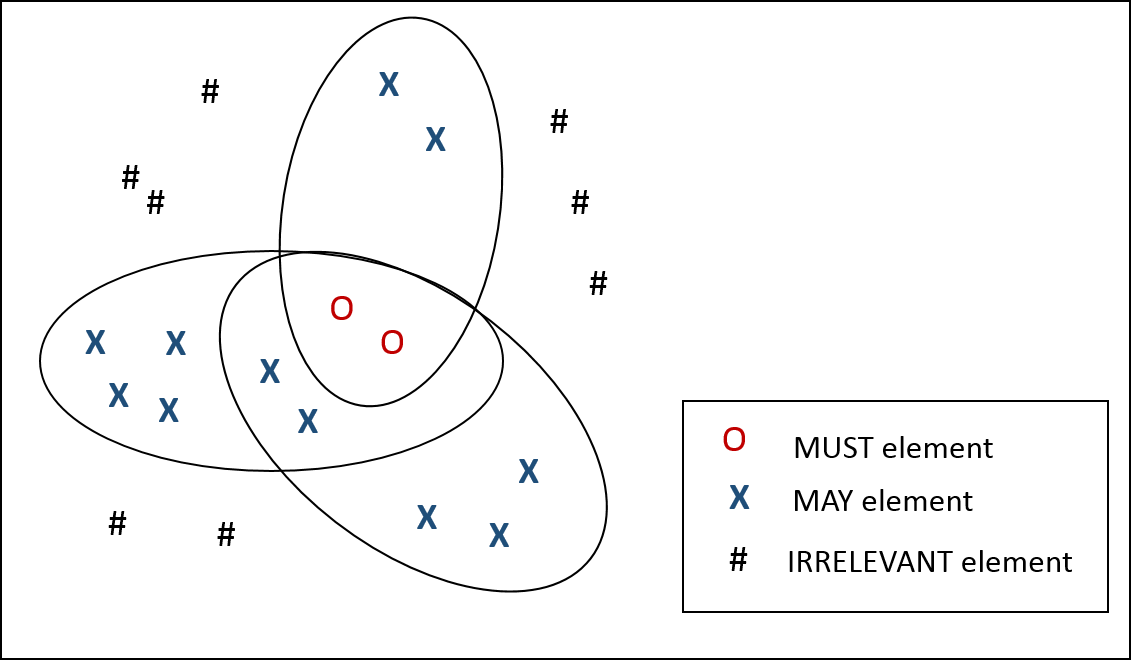
\includegraphics[width=\columnwidth]{figs/may_must.png}
%\caption{A visual example of partitioning the implementation model}\label{fig:maymust}
%\end{center}
%\end{figure}

\iffalse
In light of this intuition, we define existing coverage notions in the literature, which are based on the idea of \emph{mutation}. Then, later, we explore some novel notions of coverage based on the idea of support sets.  More formally, mutation, denoted by $f_m$, is a relation that maps $\Gamma$ to set $S \subset \Gamma$ (written as $f_m (S)$). The range of $f_m$ for $\Gamma$ is denoted by $M$.

In general, requirements completeness can be defined with regard to the notion of \emph{coverage}. In fact, the way that coverage is formalized plays a key part in the strength/ effectiveness of a method for the assessment of completeness. Requirements completeness can be judged on a fraction called \emph{coverage score}, the closer to 1 the score is, the more complete the specification is.

\begin{definition}{\emph{Coverage:}}
  \label{def:coverage}
   Any notion of coverage can be formalized as a function $\psi$ such that,
   $\forall r \in \Delta, \varphi \in \Gamma$, if $\varphi$ is covered by $r$ then $\psi (r, \varphi) = true$, denoted by $\psi (r) \preccurlyeq \varphi$, otherwise  $\psi (r, \varphi) = false$, denoted by $\psi (r) \nprec \varphi$.
\end{definition}

\begin{definition} {\emph{Coverage based on single mutation \cite{chockler2010coverage, chockler_coverage_2003}:}}
  \label{def:coverage1}
   $\forall r \in \Delta$,
   $\varphi \in \Gamma$,
   $\psi (r) \preccurlyeq \varphi$
   iff $\Gamma \vdash r$ and
   $f_m (\Gamma \setminus \{ \varphi \}) \nvdash r$. Otherwise, $\psi (r) \nprec \varphi$.
\end{definition}

For the sake of simplicity, we refer to the coverage function
formalized in Definition \ref{def:coverage1} as $\psi_{sm}$.
Back to our example, $\psi_{sm}$ only considers {\tt P} and {\tt c3} as covered in the model shown in Fig. \ref{fig:ex}.

Using $\psi_{sm}$, the coverage score of specification $r$ is computed by $$\frac{\sum_{\varphi \in \Gamma} f_m (\Gamma \setminus \{ \varphi \}) \nvdash r}{|\Gamma|}$$
Usually, a mutation is an atomic change to the design whose effect is not masked by other modifications, which means simultaneous mutations may result in masking the changes. However,
it is possible to define the coverage notion with regard to all possible mutations, although it would be also very expensive and impractical \cite{chockler2001practical}. \ela{Mike, is the citation correct?}.
For a coverage function based on all mutations, the coverage score is calculated by
$$ \frac{\sum_{S \in M} f_m (S) \nvdash r}{|\Gamma| |M|}$$
\fi
\fi





\section{Coverage Analysis and Requirements Completeness}

For critical systems, it has been argued that formal methods
%, involving formalized requirements and proofs of implementation correctness,
should be applied to gain higher assurance than is possible with testing~\cite{Miller10:CACM,Rushby09:SEFM,Hardin09:Security}.  For these approaches, testing may still be performed, but the verification effort is primarily focused on performing proofs.  Unfortunately, proof-based approaches tend not to answer the question as to whether implementations have {\em additional functionality} that is not covered by requirements.  %Testing, despite its faults, can measure {\em structural coverage} to find untested functionality and can find some errors by {\em serendipity}, in which problems not directly related to the requirement under test are exposed.  Therefore, in formal verification approaches, it is even more important that requirements be complete.
%
Thus, we are interested in notions of {\em coverage}: determining how well the requirements characterize the implementation model.
The goal of a {\em coverage metric} is usually to assign a numeric score that describes how well properties cover the design.

Relatively recently, techniques have been devised for analyzing completeness of requirements against formal implementation models, specified as transition systems or Kripke structures \cite{chockler2001practical,das2005formal, claessen2007coverage, grosse2007estimating,chockler_coverage_2003,chockler2010coverage,
Kupferman:2006:SCF,kupferman_theory_2008}.  These models are agnostic to the abstraction level of the implementation: implementations can be lower-level requirements, software architectures, or concrete implementations of system behavior.  The mechanism used is based on {\em mutation} and {\em proof}: is it possible to prove that the requirements still hold of the system after mutating the model in some way?  If so, then the requirements are incomplete with respect to that model element.


\iffalse
Mutations are ``atomic'' changes to the design, where the set of possible mutations depends on the notation that is used.  A mutant is ``killed'' if one of the properties that is satisfied by the original design is violated by the mutated design~\cite{chockler_coverage_2003,chockler2001practical,chockler2010coverage,Kupferman:2006:SCF,kupferman_theory_2008}.  There are many different kinds of mutations that have been proposed, primarily focused on checking sequential bit-level hardware designs.
For these designs, {\em State-based} mutations flip the value of one of the bits in the state.  There are several variations depending on whether the flip is performed on a single state within a Kripke structure~\cite{hoskote1999coverage}, or in the description of the signal in the transition relation of the circuit~\cite{chockler2001practical}.  {\em Logic-based} mutations fix the value of a bit to constant zero or one, and can be used to determine whether properties can find stuck-at faults.  {\em Syntactic} mutations~\cite{chockler_coverage_2003} remove states in a control flow graph representation of hardware.
Similarly, for software, it is possible to apply any of the ``standard'' source code mutation operators used for software testing~\cite{Andrews06:mutation} towards requirements coverage analysis.
Some examples of software mutations are \cite{Budd:1980}:
\begin{enumerate}
    \item Replace an integer constant $C$ by one of $\{0, 1, -1, C + 1, C - 1\}$,
    \item Replace an arithmetic, relational, logical, bitwise logical, increment/decrement, or arithmetic-assignment operator by another operator from the same class,
    \item Negate the decision in an \texttt{if} or \texttt{while} statement,
    \item Delete a statement.
\end{enumerate}

We assume each element $T_i \in T$ has a set of possible mutations associated with it.  Depending on the modeling formalism used, this may be the value of a gate or signal or an expression within a statement in a program.  We will further assume the existence of a mutation function $f_{m}$ that, given a model element, will return a finite set of mutations for that element.  We can then define the set of mutant models $M$ as follows:
\[
    M = \{ (T \setminus \{T_i\}) \cup \{m\} \ |\ T_i \in T, m \in f_{m}(T_i) \}
\]
\noindent and then define the mutation score for property $P$ in the standard way:
\begin{definition} {\emph{Generalized mutation coverage.} } \\
\[
   \mutcov = \frac{ | \{m~|~ m \in M~\land~(I, m) \nvdash P\} |}{|M|}
\]
\end{definition}

\noindent Note that without loss of generality, we consider a single property $P$, which can be viewed as the conjunction of all the properties of the model.

The state of the art of mutation-based coverage can be found in Chockler \textit{et al.} \cite{chockler2010coverage}, where a design is considered as a net-list with nodes of types {\small \texttt{\{AND, INVERTER, REGISTER, INPUT\}}}.
Each mutant design changes the type of a single node to {\small \texttt{INPUT}}. When property $\phi$ satisfied by the original net-list fails on the mutant design, it is said that a mutant is discovered for $\phi$. Then, the coverage metric for $\phi$ is defined as the fraction of the discovered mutants, based on which the coverage of a set of properties is measured as the fraction of mutants discovered by at least one property.
To decrease the cost of computation, coverage analysis is performed at several stages; first, all the nodes that do not appear in the resolution proof of a given property are marked as \emph{not-covered}, and the rest of the nodes are marked as \emph{unknown}. Then, for the unknown nodes, the basic mutation check is performed: if a corresponding mutant design violates the property, it will be considered as \emph{covered}.
\fi

Unfortunately, previous metrics based on mutation are expensive to compute, as they involve running many different verification efforts against mutant models.  For example, given a mutant generator developed for testing Lustre programs~\cite{jkind}, the 50 largest models in the benchmark suite each had more than 30,000 mutants.  While it is possible to approximate mutation coverage scores using sampling~\cite{Zhang13:sampling}, samples still often require 5\% or more of the possible mutants.  One can also restrict the set of possible mutations, but this runs the risk of biasing the program to miss certain kinds of faults.

Thus, we propose a new family of metrics for measuring property completeness based on proofs and \mivc s rather than mutation.  These metrics are based on the notions of \mivc s and MAY and MUST elements introduced in the previous section.  The metrics have benefits in that they are cheaper to compute than previous metrics (especially the \mivc\ metric) and have a formal basis provided by proofs.

For the purposes of this discussion of coverage, without loss of generality, we assume that the analysis is performed over a single property $P$ (which may represent the conjunction of all of the properties for the model).

%they can {\em underapproximate} the portion of the model necessary for proof
%can {\em underapproximate} which portions of an implementation model are necessary to produce a proof.
%completeness metrics can {\em underapproximate} which portions of a program are necessary to fulfill the requirements.  That is, if we construct a model consisting of only the required model elements as determined by the analysis, it is often no longer possible to prove the requirement.  Thus the feedback provided to the developer may be somewhat misleading.  In addition, the mutation-based analyses tend to be very computationally expensive.  For example, for model checkers, state of the art techniques have runtimes of (in the best case) several times more than is required for proof~\cite{chockler2010coverage}.


%\footnote{Section~\ref{sec:impl} describes how these proofs are discovered in practice.}
%\subsection{Coverage and Minimal Proofs}
%Alternatively, we can consider using the proofs themselves as a mechanism for determining adequacy of requirements.

\begin{definition} {\emph{IVC coverage (\ivccov):}} \\
\label{def:coverage-justi}
Given $S \in \aivc(P)$, $T_i$ is covered by $P$ via $S$ \emph{iff} $T_i \in S$.
\end{definition}

%We call Definition \ref{def:coverage-justi} a \emph{proof-preserving} metric because, with a set of the model elements marked as covered by \ivccov ,
%$P$ is provable.  %Other notions, as will be discussed,
%may yield subsets of the model that are insufficient to
%reconstruct the proof of the property.
%\footnote{\noindent ~Throughout the paper, when a coverage metric is justifiable, like \ivccov, we say that it preserves provability of the property.}
%Thus, the coverage score for \ivccov\ is often higher than the score for \nondetcov.
The coverage score for \ivccov\ can be calculated with: $$\frac{|S|}{|T|}$$  where $|T|$ is the number of conjuncts in $T$.
%Note that because minimal proofs are not unique, there are several possible coverage scores.
Because $P$ may have multiple \mivc s,
  \ivccov\ metric can lead to various scores that belong to the following set:
\[
\left\{~\frac{ |S|}{|T|}~\bigg|~S \in AIVC(P)~\right\}
\]

\noindent Note that if an \mivc ~contains all model elements (i.e., the model is {\em completely covered}), then there is only one possible \mivc , so in this case there is no diversity of scores. On the other hand, a set of states and signals can be considered covered or not covered depending on a particular \mivc\ we consider for coverage evaluation. To address this issue, we introduce additional coverage metrics using the notions of \may\ and \must.

%Since the primary goal of
% this paper has been to provide a complementary coverage notion in
%  formal verification, it is worth exploring other possible notions based on the idea of provability and $\aivc$, which is beneficial, as with testing, because if a coverage notion is an over-approximation, when the coverage
% is high, it does not necessarily mean the quality of
% the specification (or test suite) is high, or when it is an under-approximation, a low coverage score does not always mean the specification is of poor quality.

\begin{definition} {\emph{(\maycov):}}
  \label{def:comp-1}
 $T_i \in T$ is covered by $P$ \emph{iff} $T_i \in \maycov (P)$, where
   $\maycov (P) = \{T_i ~|~ \exists S \in \aivc(P)~.~T_i \in S \}$.
\end{definition}

\begin{definition} {\emph{(\mustcov):}}
  \label{def:mustcov}
 $T_i \in T$ is covered by $P$ \emph{iff} $T_i \in \mustcov (P)$, where
   $\mustcov (P) = \{T_i ~|~ \forall S \in \aivc(P)~.~T_i \in S \}$.
\end{definition}

The $\maycov$ notion considers a model element covered if it is found in any \mivc ; thus it is a weaker notion of coverage for models with multiple \mivc s, but has the benefit of being uniquely defined.  \mustcov\ takes the opposite view, considering a model element as covered only if it affects all the proofs of $P$.

\iffalse
Algorithm \ref{alg:must} is also an efficient way of computing the \emph{must} set of a given property using \ucalg. A different algorithm for computing $\must (P)$ is to first compute $\aivc (P)$ and then take the intersection of all sets in $\aivc (P)$.


\begin{algorithm}
  \SetKwInOut{Input}{input}
  \SetKwInOut{Output}{output}
  \Input{$(I, T) \vdash P$}
  \Output{Must set for $(I, T) \vdash P$}
  \BlankLine
  $S \leftarrow \ucalg((I, T) \vdash P)$ \\
  $M \leftarrow \varnothing$ \\
  \For{$x \in S$} {
    \If{$(I, T\setminus\{x\}) \nvdash P$}{
      $M = M \cup \{x\}$
    }
  }
  \Return{M}
\caption{\mustalg: an algorithm to compute $\must(P)$ for a given $P$}
\label{alg:must}
\end{algorithm}
\fi

\iffalse
It is still possible to build more relaxed coverage metrics in which coverage
is captured by looking at individual properties, rather than their conjunction.
%for example, in the definition of \ivccov , it is wise to look at $P$ as
%the conjunction of all properties. However,
We can, for example, describe a metric in which any element used by an \mivc ~for any property is considered covered.
%with this view,
%elements around IVCs that do not have common \emph{must}
%elements with others will be treated as uncovered while they are at least covered by one
% IVC of an individual property in the specification.
%
The next definition, \allcov, formalizes this notion.
\begin{definition} {\emph{(\allcov):}}
  \label{def:comp-2}
     Given a set of properties $\Delta$ over $T$, $T_i \in T$ is covered
   \emph{iff} $T_i \in \allcov (T)$, where
   $\allcov (T) = \{T_i ~|~ \exists P \in \Delta ,~ S \in \aivc(P).~T_i \in S \}$.
\end{definition}

\fi

\iffalse
Based on the categorization of elements, we will state a relationship about \mivc s in order to compare different proof-based metrics proposed earlier.

\begin{lemma}
  \label{lem:must-not-enough}
  If $\may(P) \neq \varnothing$, then $P$ is not provable by $\must(P)$.
\end{lemma}
\begin{proof}
  $\may(P) \neq \varnothing \Rightarrow  \exists T_i \in \may(P).$
$T_i \in \bigcup \aivc(P) \wedge T_i \notin \must(P)$,
which implies $\exists S \in \aivc(P).~ T_i \in S$.
Considering the fact that $S$ is minimal and
$\must(P) \subset S$ (since $T_i \in S \wedge T_i \notin \must(P)$),
 $\nexists S' \subset S.~ (I,S') \vdash P$,  which means $(I, \must(P)) \nvdash P$.
\end{proof}
\vspace{2mm}

\fi

%\begin{lemma}
%    \label{lem:must-mustcov}
%    $T_i \in \must(P) \Leftrightarrow T_i \in \mustcov(P)$
%\end{lemma}
%\begin{proof}
%Immediate from the definition of $\must$ and \mustcov.
%\end{proof}

\iffalse
Now we focus on the relationship between non-deterministic mutation-based coverage and proof-based metrics. In Chockler et. al.
~\cite{chockler2010coverage},
each mutant design changes the type of a single node to an input node .
Given a suitable encoding of the netlist, assigning a ``fresh'' input is an isomorphic operation to simply removing a $T_i$ from $T$. The mapping is as follows: the net-list becomes a conjunction
of equations, where each vertex becomes a variable $v_i \in U$, and where each non-input vertex becomes an assignment equation $T_i \in T$.
For example, given an AND-vertex $v_i$ with three input edges from other vertexes $\{v_a, v_b, v_c\}$, we would define an equation $T_i \in T$ of the form $(v_i = (v_a \wedge v_b \wedge v_c))$.
%
%As the variable is no longer constrained by a defining equation, it is effectively an %input.

Given this encoding, we can reframe the non-deterministic coverage proposed in \cite{chockler2010coverage} as follows:

\begin{definition} {\emph{Nondeterministic coverage (alternate specification) (\nondetcovalt) ~\cite{chockler2010coverage}.} }
\label{def:non-det-2}
$T_i \in T$ is covered by property $P$ \emph{iff} $T_i \in \nondetcovalt (P)$, where
$\nondetcovalt (P) = \{T_i~|~ (I, T) \vdash P \wedge (I, T \setminus \{T_i\}) \nvdash P\}$.
\end{definition}
\noindent Given this definition, it becomes straightforward to define some additional properties.

\begin{lemma}
  \label{lem:must-coverage}
$T_i \in \nondetcovalt (P) \Leftrightarrow T_i \in \mustcov(P)$.
\end{lemma}
\begin{proof}
$T_i \in \nondetcovalt (P)$ means that $(I, T \setminus \{ T_i \}) \nvdash P$ then
%$T_i$ is necessary to prove $P$,  which means
$\forall S \subset T .~ T_i \notin S \Rightarrow (I, S) \nvdash P$.
Therefore, since $(I, T) \vdash P$, $T_i \in \bigcap \aivc(P)$, which means  $T_i \in \must(P)$.
On the other hand, let $T_i \in \must(P)$; then $\forall S \in \aivc(P).~ T_i \in S$.
By definition, any proof of $P$ is a superset of some minimal IVC in $\aivc(P)$.
Thus, any subset $S$ of $T$ leading to proof contains $T_i$.
Therefore, $T \setminus \{ T_i \}$ does not lead to a proof.

\end{proof}
\vspace{2mm}

In light of Lemma \ref{lem:must-coverage}, the \nondetcovalt\ coverage score of specification $P$ can be also calculated by
$$\frac{|\must(P)|}{|T|}$$
%Therefore, for set of properties $\Delta$, the coverage score is computed by $$\frac{|\must(\Pi)|}{|T|},\quad  \Pi= \bigwedge_{i} {P_i \in \Delta}$$


%\mike{after all metrics presented, contrast them on the example.  Introduce the properties HERE and then discuss the coverage sets}
%
%\mike{Then, you can talk about justification, etc.}
\begin{corollary}
\label{cor:must-not-provable}
\nondetcovalt\ is not proof-preserving.
\end{corollary}
\begin{proof}
Immediate from Lemma \ref{lem:must-not-enough} and Lemma \ref{lem:must-coverage}
\end{proof}
\vspace{2mm}
\begin{corollary}
\label{cor:ivc-provable}
\ivccov\ is proof-preserving.
\end{corollary}
\begin{proof}
Immediate from Definition~\ref{def:minimal-ivc} and Definition \ref{def:coverage-justi}
\end{proof}
\vspace{2mm}

%It should be pointed out that \ivccov\ is accurate meaning that it does not result in false positives. In other words, since IVCs are \emph{minimal}, \ivccov\ does not mark
%any \emph{actual} uncovered element as covered.
\fi

\iffalse
Figure~\ref{fig:runtimeall} allows a visualization of the runtime of different coverage analyses
in comparison with the proof time, which indicates the overhead induced by each algorithm.
As can be seen, it is computationally cheap to find an
approximately minimal IVC using the algorithm \ucalg; however, finding a {\em guaranteed}
minimal IVC using the \ucbfalg\ algorithm is computationally expensive. The overhead of the \ucalg\ algorithm is on average 31\% over the baseline proof, as opposed to 2276\% for the \ucbfalg\ algorithm.
Therefore, in order to compute \ivccov, it is much more efficient to use \ucalg\ rather than the \ucbfalg\ algorithm.
In terms of comparing cost of coverage computation from \ivccov\ and \mustcov ,
the \mustcov\ computation imposes an average 4183\% runtime overhead on the verification time.
\fi

\iffalse
\begin{figure}
  \centering
  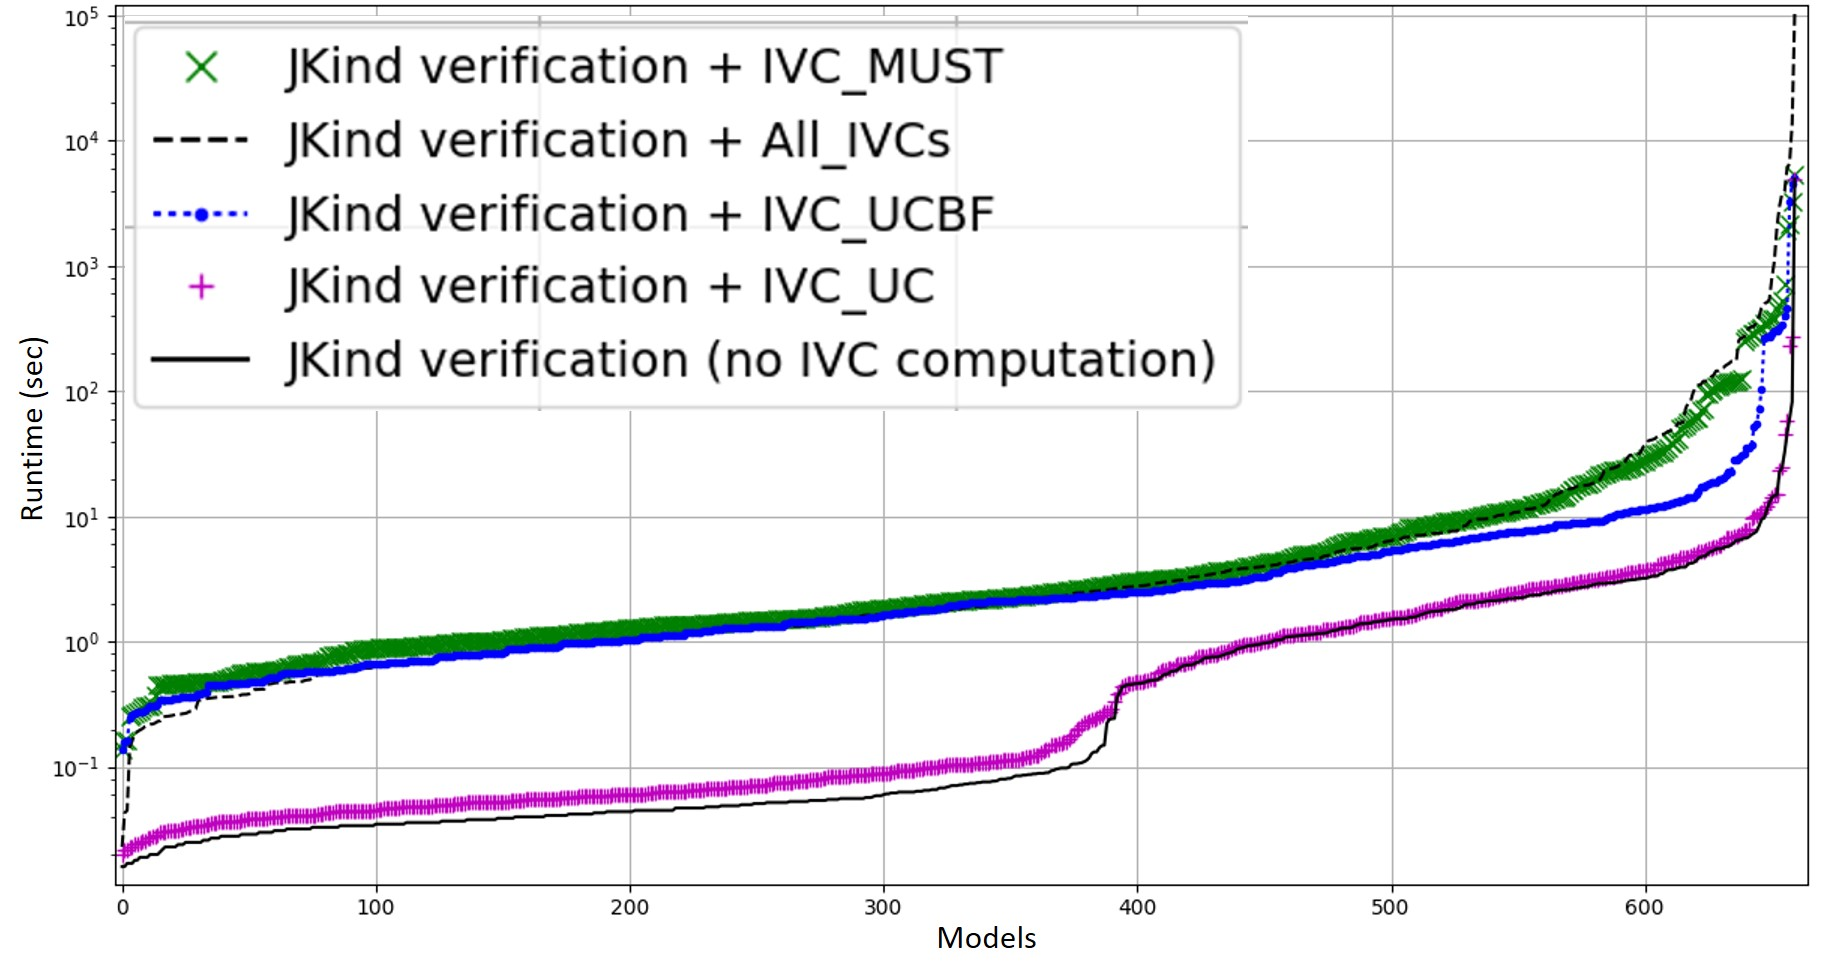
\includegraphics[width=\columnwidth]{figs/timing_cv.jpg}
  %\vspace{-0.2in}
  \caption{Runtime of different analyses}\label{fig:runtimeall}
\end{figure}
\fi

\begin{figure}
  \centering
  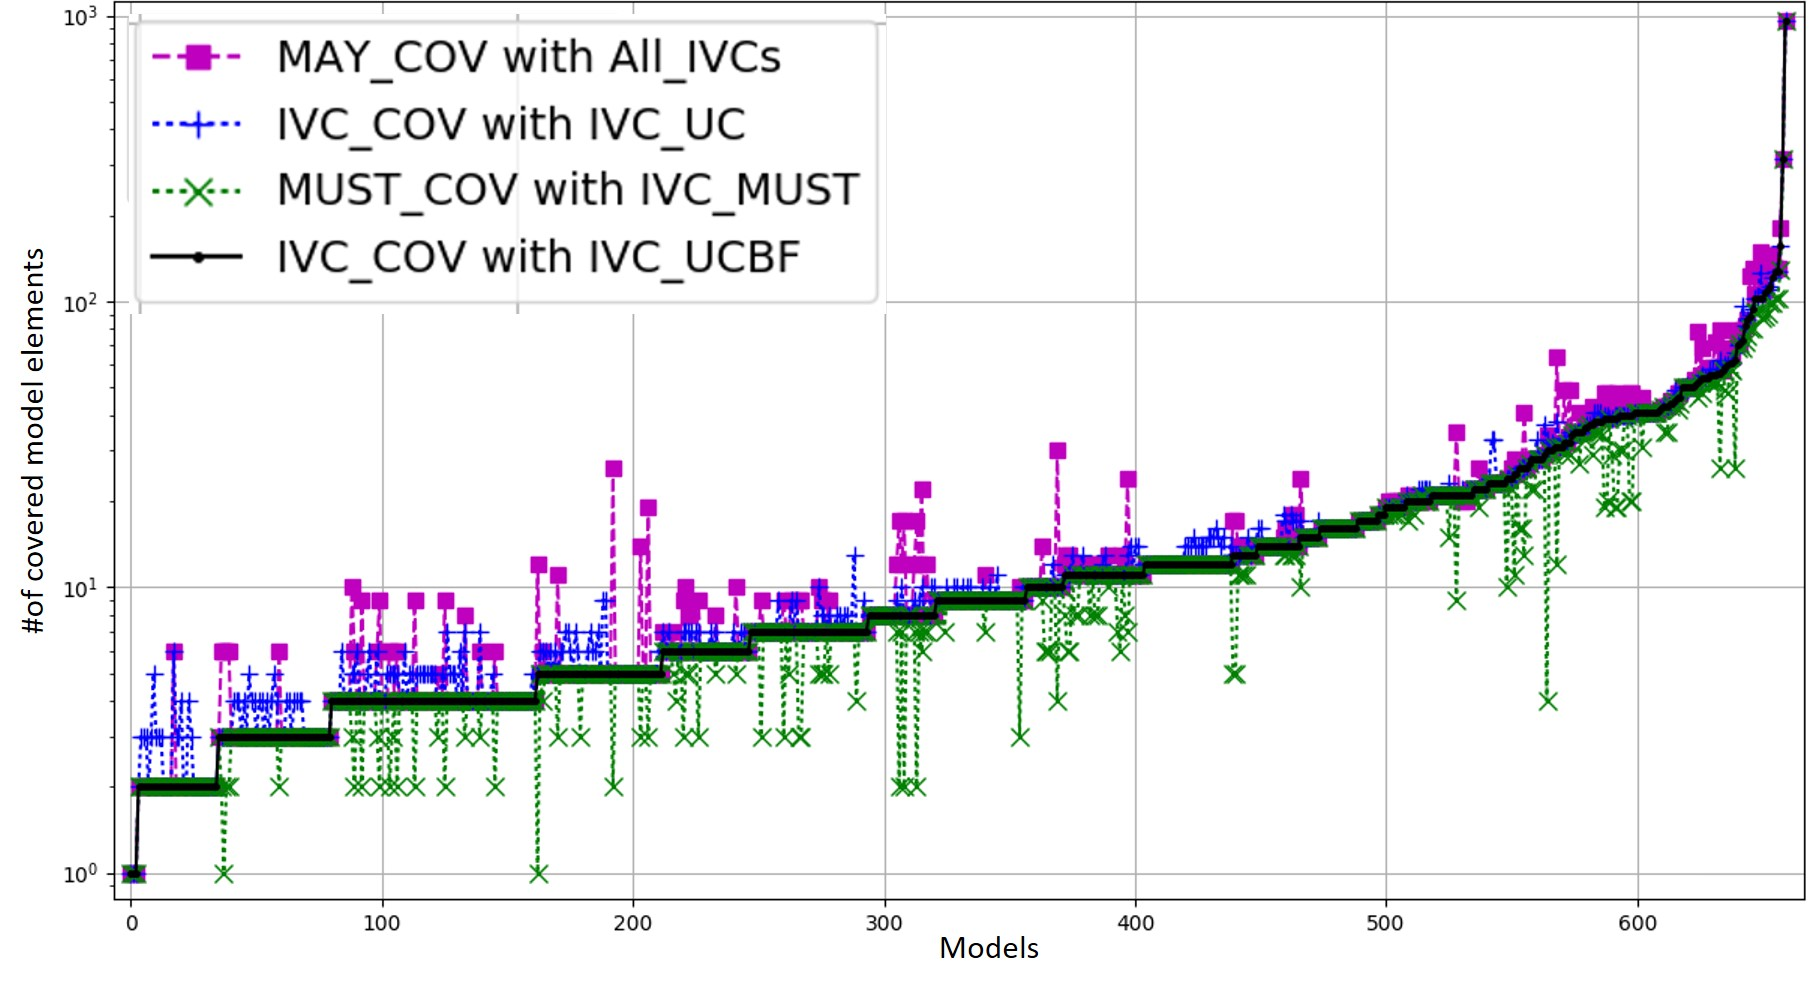
\includegraphics[width=\columnwidth]{figs/cv_size.jpg}
  %\vspace{-0.2in}
  \caption{Size of the set of covered elements by different algorithms}\label{fig:cvsize}
\end{figure}

When a coverage metric brings about lower coverage scores on average,
we say that the metric is harder to satisfy. To study this aspect of the proposed metrics, we first calculated the size of the output sets generated by each algorithm: on average, the ratio of the size of the sets generated by \ucalg\ to the size of the ones obtained from \ucbfalg\ is 1.08,
while this ratio for \mustalg\ to \ucbfalg\ is 0.93, which shows \mustalg\ is harder to satisfy.

Figure \ref{fig:cvsize} is a visualization of the size of the set of covered elements by different algorithms. Models over the x-axis are sorted based on the size of the minimal IVCs obtained from the \ucbfalg\ algorithm.  The graph shows the degree of under-approximation of a minimal proof set by \mustcov\ as well as the degree of over-approximation by \ucalg\ and \maycov.  The proposed coverage metrics can be ranked in terms of their scores as follows:
$$\mustcov \leq \ivccov\ \leq \maycov\ $$
\ivccov\ and \mustcov\ are equivalent when all elements within the model are covered.  If all model elements are part of an \mivc, then there is only one \mivc\ possible and all elements are \must\ elements.

%The equivalence of \mustcov\ and \nondetcovalt\ allows us to compare our algorithms against state-of-the-art mutation based coverage.


%For many analysis problems, this may be accurate enough to

%, which makes \ucalg a reasonable choice for computing \ivccov ~(rather than using \ucbfalg ).
%Therefore, minimality does not dramatically
%affect the coverage scores when \ivccov\ is computed by the \ucalg\ rather than \ucbfalg.
%However, \ucalg might report some elements as covered, while they are not because of the minimality issue.
%And, \mustalg reports some elements uncovered, while they are because it is not able to find \emph{may} elements.

Table~\ref{tab:cov-score} describes the aggregate of the coverage scores returned by the analyses.  Across all benchmarks, the min and max coverage scores are the same, and as expected, the average number of elements required is smallest for the \mustalg\ algorithm and largest the for \ucalg\ algorithm.
One interesting point is that the coverage scores obtained from \maycov\ are not always higher than the scores computed by \ivccov.  Most of the models in our benchmark have only one \mivc. The \ivccov\ score for these models are calculated from the output of the \ucalg\ algorithm, which is not necessarily minimal. However, \maycov\ coverage scores are calculated from the output of \aivcalg\ algorithm, where minimality is guaranteed. Therefore, for the models with \emph{one} \mivc , sometimes \maycov\ yields lower coverage scores as apposed to \ivccov , which balances out the average scores by these metrics (Table \ref{tab:cov-score}).



\begin{table}
  \caption{Coverage scores of different algorithms across all models}
  \centering
  \begin{tabular}{ |c||c|c|c|c| }
    \hline
     score & min & max & mean & stddev \\[0.5ex]
    \hline\hline
    \small{\ivccov}\ with \ucalg &   0.002  & 1.0  & 0.475 & 0.302 \\[0.5ex]
    \small{\ivccov}\ with \ucbfalg&  0.002 & 1.0 &  0.445 & 0.291 \\[0.5ex]
    \mustcov & 0.002 & 1.0 &  0.417 & 0.291 \\[0.5ex]
    \maycov& 0.002 & 1.0 &  0.476 & 0.301 \\[0.5ex]
    \hline
  \end{tabular}
  \label{tab:cov-score}
\end{table}


\iffalse
To investigate the relationship between provability and different coverage notions,
we were interested in the number of models in the benchmark for which
\mustalg\ resulted in the sets not equal to an MIVC (i.e. models for which
\mustalg\ did not preserve provability).
Obviously properties are provable by 100\% of the IVCs computed by \ucalg\ (and \ucbfalg).
As for the \mustalg\ algorithm, the properties of 290 models in the benchmarks were not provable by the output of \mustalg. In practice, for larger models, \mustcov\ is more likely not to maintain provability,
 and since more than half of the models are small, 43\% may still not reveal the actual degree
 to which \mustcov\ underapproximates the covered parts of a model.
  The notion of proof preservation is appealing because it allows a concrete demonstration to the user of the irrelevance of portions of the implementation.  The IVC coverage notion also allows, in cases where there are multiple minimal satisfying sets, insight on multiple ways by which the model meets a requirement.
\fi

%To conclude this section, we should mention that one can define many more proof-based coverage metrics based on the $\mivc$s and $\aivc$s.  Metrics that make use of the $\aivc$ relation are computationally more expensive than \ivccov.


\iffalse
The size of sets computed by \ucalg\ is very close to the size
of the ones obtained from \ucbfalg, especially for larger models.  The average increase in size of IVCs returned by \ucalg\ is approximately 8\% of the \ucbfalg\ algorithm.  Since the overhead of producing \ucalg\ is only approximately 31\% more expensive than the baseline analysis, this test may be efficient enough to run as a standard part of the model checking process.  %If guaranteed minimality is required, the \ucbfalg\ can be used, but
\fi




%\subsection{Optimizing Logic Synthesis}

\input{synthesis}
